\documentclass[12pt]{report}
\usepackage{indentfirst}
\usepackage{geometry}
\usepackage{flafter}
\usepackage{graphicx}
\usepackage{float}
\usepackage{titlesec}
\usepackage{tabularx}

\graphicspath{ {./images/} }
\newgeometry{vmargin={15mm}, hmargin={30mm,30mm}}
\titleformat{\chapter}{\normalfont\huge}{\bf\thechapter.}{18pt}{\huge\bf}

\begin{document}

\begin{titlepage}
    \vspace*{4cm}
    \rule{\textwidth}{2px}

    \begin{center}
        \textbf{\huge{{Summer Practice Report }}}\par \vspace{0.2cm}
        \textbf{\Large{{TÜBİTAK İLTAREN}}}\par
    \end{center}
    
    \rule{\textwidth}{2px}
    
    \vspace{1cm}
    
    \begin{center}
        \large{Ahmet Eren Çolak - 2587921}
    \end{center}

    \vspace{1.3cm}
    
    \vfill
    \today
    
\end{titlepage}

\tableofcontents
\listoffigures
\listoftables

\chapter{Description of the Company}

    \section{Company Name}
    Scientific and Technological Research Council of Türkiye, Advanced Technologies Research Institute \\
    (TÜBİTAK İLTAREN)
    \section{Company Location}
    Ümitköy, 2432. Cad. 2489. Sok. Şehit Mu. Kur. Yzb. İlhan TAN Kışlası,
    Çankaya, Ankara 06800,
    Turkey.
    \section{Organizational Structure of the Company}

    \begin{figure}[h]
        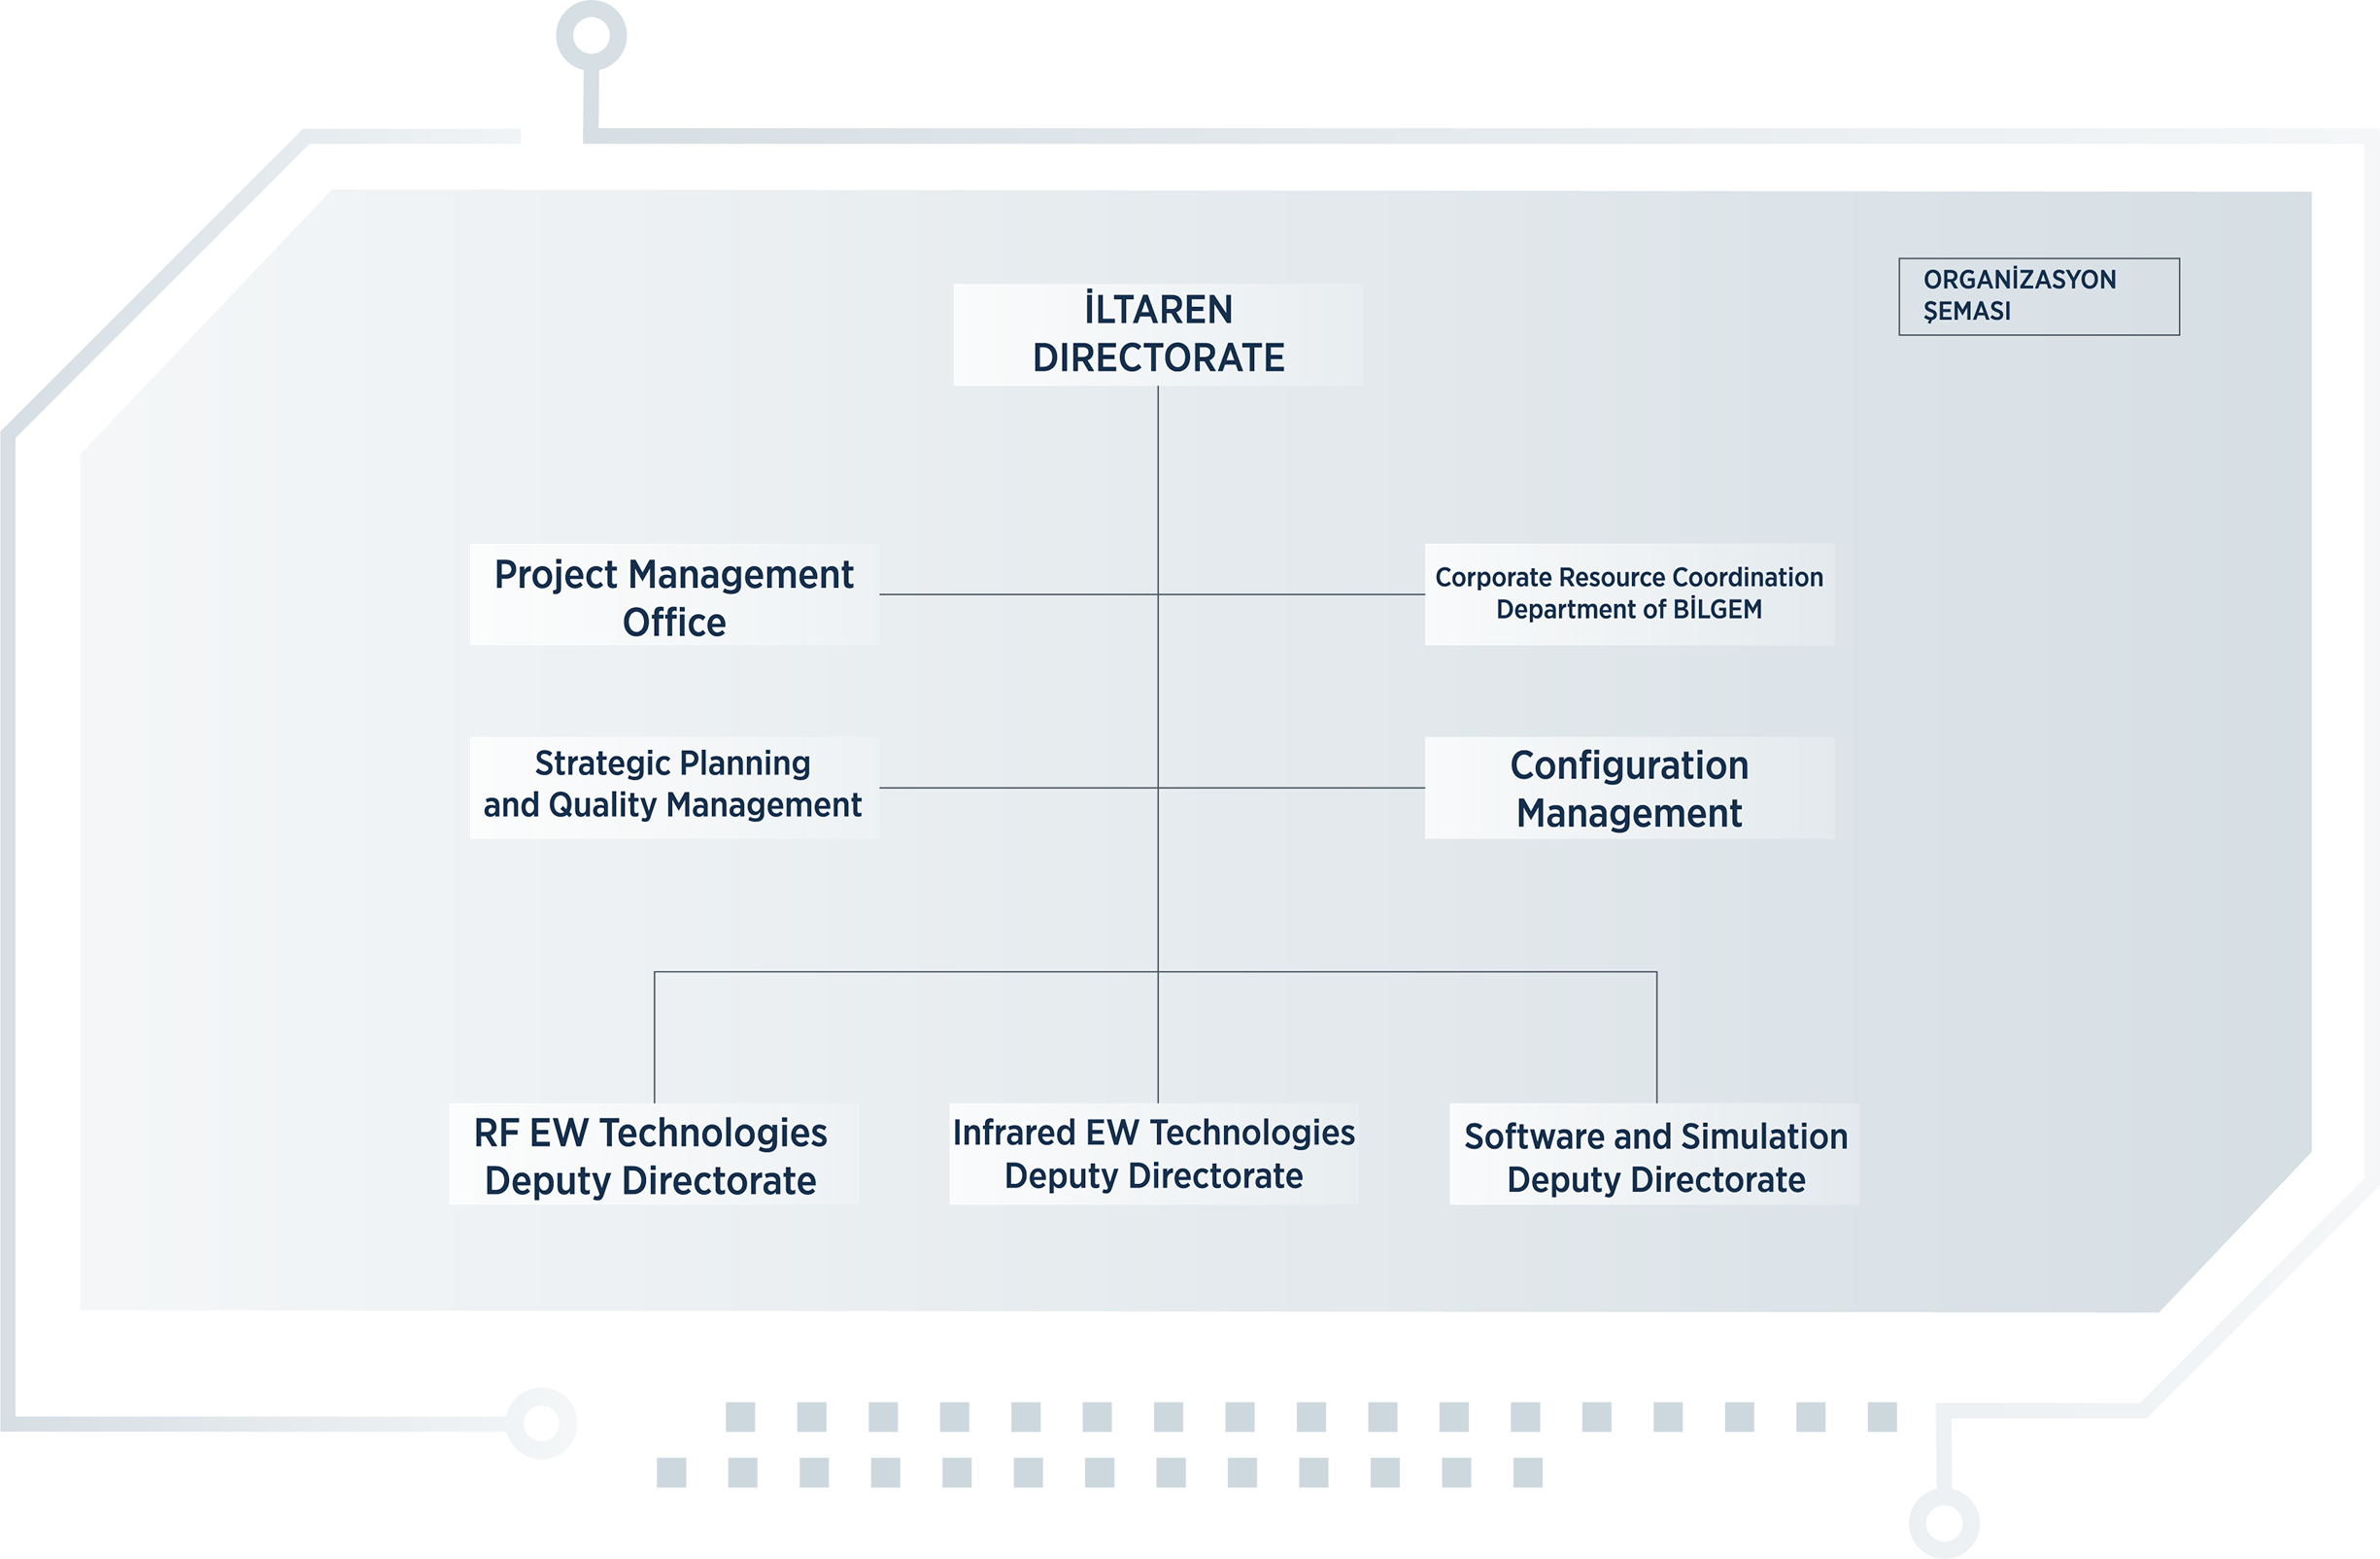
\includegraphics[scale=0.18]{iltaren-organization}
        \centering
        \caption{Organizational structure}
    \end{figure}

    \section{Number and Duties of Engineers Employed}
    Duties and number of employees can not be shared due to confidentiality policies of the company.
    \section{Main Area of Business}

    Advanced Technologies Research Institute (İLTAREN) performs the tasks of conducting research on all kinds of software, hardware and 
    equipment in the field of Electromagnetic Warfare, developing technologies and prototypes, creating methods and processes for developing 
    and evaluating EW techniques and tactics, creating infrastructures for testing, measurement, analysis and evaluation activities for 
    EW systems, and conducting scientific research in related fields of activity.

    \section{Brief History of the Company}
    The Advanced Technologies Research Institute (İLTAREN) is an organization based in Turkey that specializes in electronic warfare and advanced technology research. Here is a brief history of İLTAREN:
        \\ \newline
        \textbf{1999 - Establishment:} İLTAREN was established as a result of a protocol signed between the General Staff Communications Electronics and Information Systems Directorate and TÜBİTAK (The Scientific and Technological Research Council of Turkey). This protocol laid out the framework for cooperation in establishing the institute.
        \\ \newline
        \textbf{2000 - Inception:} İLTAREN officially began its activities under the TÜBİTAK Presidency in the year 2000. Its primary mission was to enhance the electronic warfare capabilities of the Turkish Armed Forces (TAF) through advanced research and technology development.
        \\ \newline    
        \textbf{2003 - Restructuring:} İLTAREN underwent restructuring, with the signing of a second protocol. It continued its operations as a unit within the National Research Institute of Electronics and Cryptology (UEKAE).
        \\ \newline
        \textbf{2007 - National Frequency Management System:} İLTAREN achieved a significant milestone with the development of the first version of the National Frequency Management System. This system is crucial for managing and allocating radio frequencies efficiently.
        \\ \newline
        \textbf{2010 - International Contributions:} İLTAREN developed the ARCADE product to meet NATO Spectrum Management needs and actively contributed to NATO Electronic Warfare exercises.
        \\ \newline
        \textbf{2011 - Infrared Trace Analysis Software:} İLTAREN developed Infrared Trace Analysis Software, which is likely a significant asset in the field of electronic warfare.
        \\ \newline
        \textbf{2012 - Engineering Support Contracts:} İLTAREN signed contracts with the Turkish Land Forces Command and NATO for engineering support in the field of electronic warfare and Spectrum Management needs, respectively.
        \\ \newline
        \textbf{2013 - İLTAREN Institute:} İLTAREN began to serve as an institute affiliated with BİLGEM (Informatics and Information Security Advanced Technologies Research Center).
        \\ \newline
        \textbf{2014 - Hardware Development:} İLTAREN continued its hardware development efforts, including the development of the Digital Tactical Simulator for Electronic Warfare self-defense.
        \\ \newline
        \textbf{2016 - Hardware In-Loop Laboratories:} İLTAREN expanded its capabilities with the development of Hardware In-Loop Laboratories for self-protection methods against both radio frequency (RF) and infrared systems.
        \\ \newline
        \textbf{2017 - Multi-Purpose Phased Array Radar Project:} İLTAREN contributed to radar technology development within the scope of the Multi-Purpose Phased Array Radar Project.
        \\ \newline
        \textbf{2018 - Instrumented Infrared Seeker Test System:} İLTAREN developed the Instrumented Infrared Seeker Test System, further advancing its expertise in infrared technology.
        \\ \newline
        \textbf{2019 - Engineering Support Agreement:} İLTAREN signed an agreement with the Turkish Air Forces Command to provide engineering support in the field of electronic warfare.
        \\ \newline
        \textbf{2020 - ESEMOD Software:} İLTAREN expanded the use of its ESEMOD software to work on MİLGEM class ships.
        \\ \newline
        \textbf{2021 - Jamming Code Development:} İLTAREN developed laboratory infrastructure for the development of jamming codes used in Directed Infrared Countermeasure Systems.
        \\ \newline
        \textbf{2022 - National Combat Aircraft Project:} İLTAREN played a role in the development of the integrated processor unit and avionic interface platform hardware for the National Combat Aircraft Project.
        \\ \newline
        \textbf{2023 - Radar Analysis Software:} İLTAREN delivered Radar Analysis Software for the National Joint Electronic Warfare Data Bank (MMEHBB) and celebrated the first functional flight of the Electronic Warfare Pod on the F16.
        \\ \newline
    Throughout its history, İLTAREN has consistently contributed to the advancement of electronic warfare technologies, Spectrum Management, and related fields, serving as a vital asset for the Turkish Armed Forces and international partners.

\chapter{Introduction}
    This report provides a summary of the work I have done and experiences I have gained during my 6-week summer 
    practice at the Advanced Technologies Research Institute (İLTAREN). 

\chapter{Project}

    \section{Analysis Phase}

    \section{Design Phase}

    \section{Implementation Phase}

    \section{Testing Phase}

\chapter{Conclusion}

\chapter{Appendix}

\end{document}